In the previous section we mentioned the red detuning away from the cavity resonance leads to optical cooling effects. We normally differ between the optimal cooling regime, i.e. resolved sidebands, and the less optimal cooling regime, i.e. unresolved sidebands. As shown in the section above vibrating mirror causes scattering of the cavity fields into sidebands $A_{\pm}$. We can use the cavity to either amplify or suppress/filter out the generated sidebands at frequency $\Omega_m$. The resolved sideband regime is reached when your cavity linewidth becomes much smaller than the mechanical resonance, i.e. $\kappa \ll \Omega_m$, as shown in figure \ref{fig:resolved_sb}. If this criteria is fulfilled the cavity can only support one generated sideband and therefore suppresses the other sideband.

\begin{figure}[H]
\centering
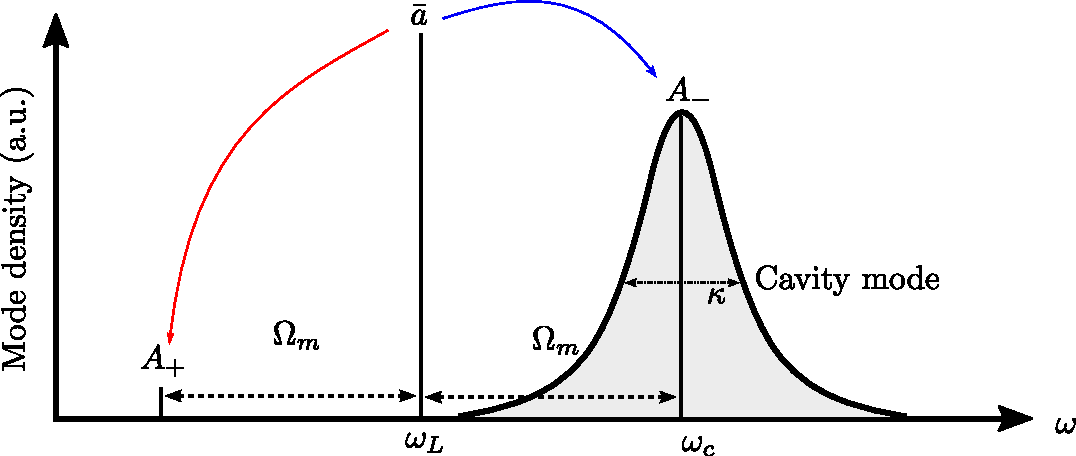
\includegraphics[scale=0.8]{resolved_sb.pdf}
\caption{Scatter picture of optimal cooling in the resolved sidebands regime. The cavity mode only supports the $A_-$ mode at frequency $\Omega_m$ detuned from the carrier and filters out the rest.}
\label{fig:resolved_sb}
\end{figure}

Moving on to describing the unresolve sidebands regime, i.e. $\Omega_m \ll \kappa$. This regime is as mentioned less optimal for cooling, since the cavity linewidth is now much larger than the mechanical resonance as shown in figure \ref{fig:unresolved_sb}. The cavity can now support both sidebands at the same time, so heating and cooling is present at the same time.

\begin{figure}[H]
\centering
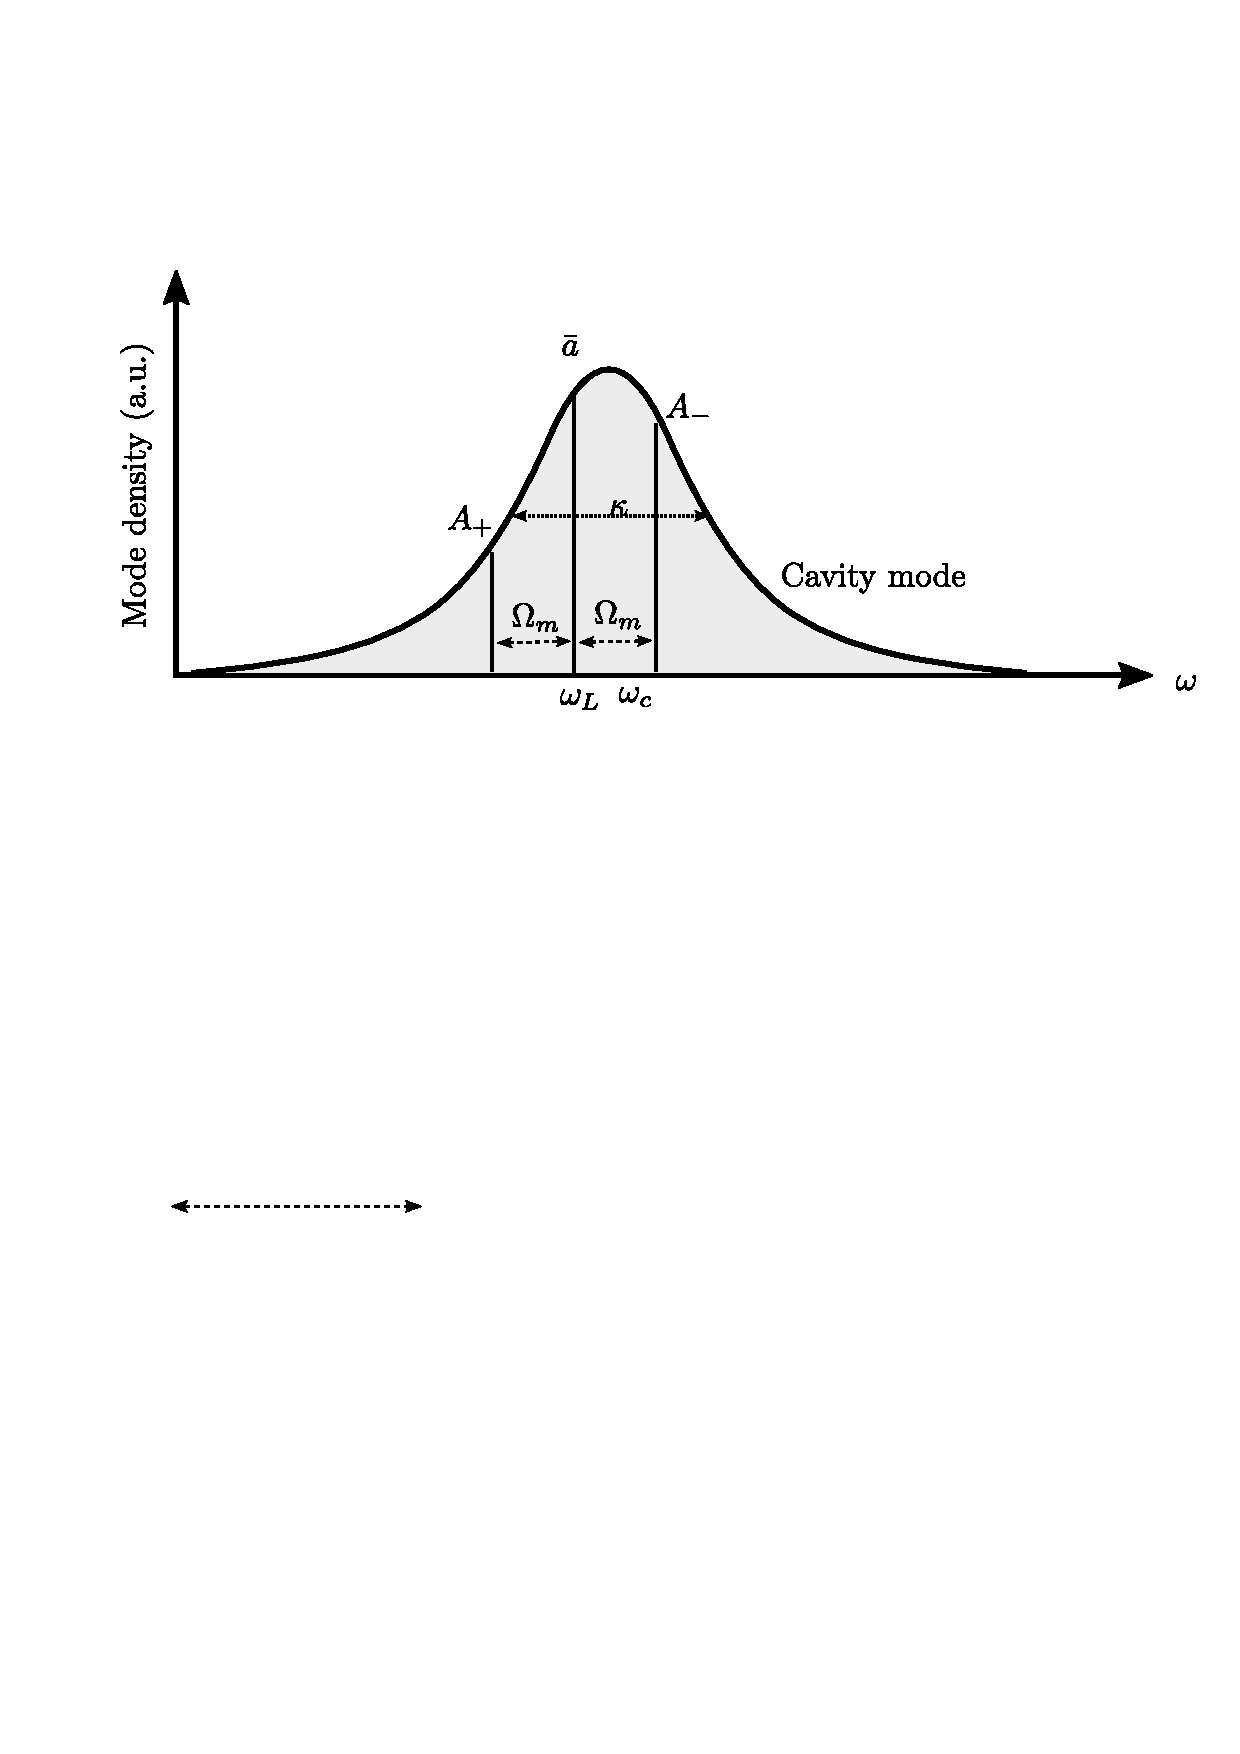
\includegraphics[scale=0.8]{unresolved_sb.pdf}
\caption{Scattering picture in the unresolve sidebands regime. The cavity resonance is now much broader than the mechanical resonance.}
\label{fig:unresolved_sb}
\end{figure}